\chapter{Metodologia}
Considerando as barreiras enfrentadas por novatos em software livre, em especial aquelas relacionadas a documentação dos projetos, propomos por meio desta metodologia um modelo de classificação que contribua com a identificação de informações relevantes a novos contribuidores em documentações de projetos de software livre . Esta metodologia é construída com base nas sugestões propostas por \citet{steinmacher@preliminary}, que evidenciam a necessidade de uma ferramenta que auxilie novatos quanto a documentação dos projetos. 

\section{Método}
O método proposto para esta pesquisa é dividido em seis etapas: A primeira etapa consiste em definir quais informações deverão ser identificadas nas documentações de projetos de software livre. Para isso, um conjunto de categorias será estabelecido. Este conjunto de categorias servirá para identificar quais informações são relevantes a novatos na documentação de projetos de software livre. A segunda etapa consistirá na seleção dos projetos que serão utilizados como amostra para identificação de tais categorias. Neste  passo, acontecerá também a extração das documentações para os projetos que forem selecionados. Para a terceira etapa, um experimento será proposto com novatos em software livre. Este experimento servirá para popular uma base de dados com parágrafos que contenham tais categorias estabelecidas na etapa anterior. Por fim, um modelo de classificação será elaborado com base nas informações coletadas durante o experimento, e os resultados das etapas anteriores serão avaliados por meio de métodos estatísticos. Na Figura \ref{fig:metodo-pesquisa} é apresentada a sequência de atividades a serem realizadas durante o método desta pesquisa.

\begin{figure}
    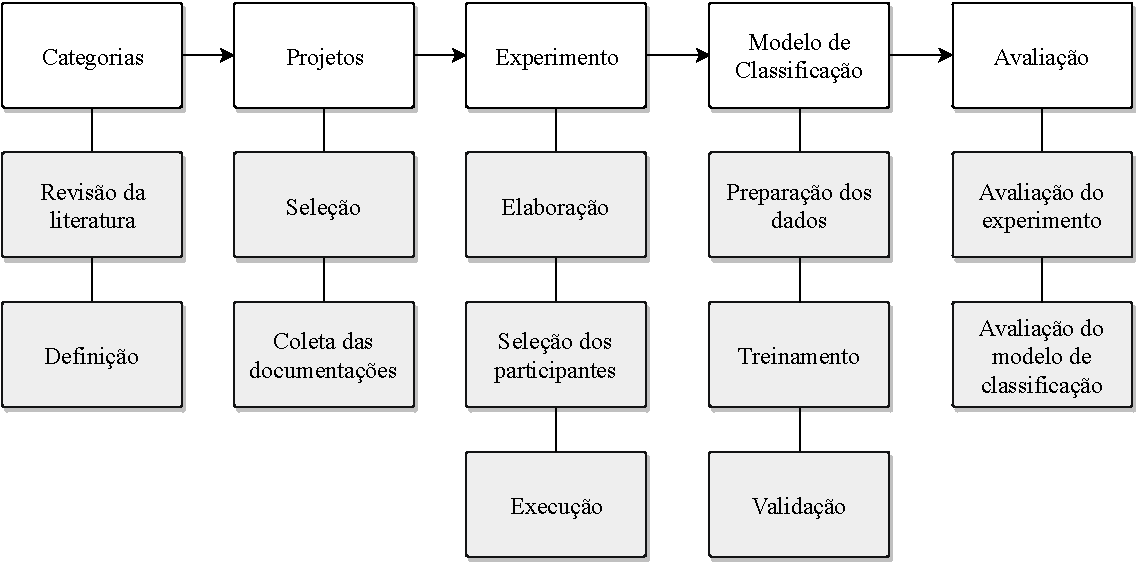
\includegraphics[width=0.9\textwidth]{figuras/metodo.pdf}
    \caption[Método de pesquisa]{Método de pesquisa. Em branco estão as principais atividades a serem executadas durante o estudo, e em cinza, as atividades secundárias de cada etapa.}
    \label{fig:metodo-pesquisa}
\end{figure}

\subsection{Categorias}
\label{sec:categorias}
Para identificar trechos nas documentações de projetos de software livre que sejam relevantes a novos contribuidores, um conjunto de categorias serão elaboradas para que seja possível realizar a identificação. Estas categorias serão estabelecidas com base nas barreiras apresentadas pelo modelo de \citet{steinmacher@preliminary}, e em demais trabalhos relacionados que identifiquem dificuldades que novatos enfrentam em software livre, em especial, estudos que identifiquem barreiras associadas a problemas de documentação nos projetos. Estas categorias servirão como identificadores dos trechos relevantes a novatos nas documentações, e serão utilizadas como as classes do experimento e do modelo de aprendizagem. 

\subsection{Projetos}
\label{sec:projetos}
Considerando que a premissa principal deste estudo é conseguir identificar trechos em documentações de projetos de software livre, um conjunto de projetos neste contexto livre será utilizado como amostra. A ideia é que os projetos sejam escolhidos a partir de um estudo proposto por \citet{avelino2015truck}, que classifica projetos populares em software livre de acordo com seu risco de sobrevivência, utilizando o \textit{fator ônibus}\footnote{O fator ônibus (do inglês, \textit{truck factor}), é uma medida de risco que investiga o quanto um determinado projeto de software depende de um número específico de pessoas. De modo geral, ele define quantas pessoas em um projeto precisam ser  ``atingidas por um ônibus'' para que o projeto fracasse ou se torne inativo.} dos projetos como métrica de avaliação. A justificativa para utilização dos projetos deste artigo está no fato de que todos contém alto índice de popularidade, estão divididos em seis linguagens de programação bem estabelecidas (JavaScript, Python, Ruby, C/C++, Java e PHP), e contém um número considerável de desenvolvedores ativos trabalhando em uma diversidade de arquivos por repositório. Como a ideia é contribuir principalmente com comunidades que necessitam de novos contribuidores, projetos que contenham \textit{fator ônibus} menor ou igual a três deverão ser selecionados. Caso o número de projetos não seja suficiente para treinar o modelo de classificação, projetos com  \textit{fator ônibus} maior do que três também poderão ser utilizados. 

De cada um dos projetos, serão extraídos os arquivos README e CONTRIBUTING dos repositórios de código, considerados por diversos trabalhos relacionados como uma das primeiras fontes de documentação apresentadas a novos contribuidores. Estes documentos serão os utilizados nas próximas etapas do estudo. A razão pela escolha destes arquivos, e não de outras fontes de documentação, se concentra no fato de que ambos apresentam informações relevantes a novos contribuidores, são de fácil extração, e são escritos escritos a partir de uma mesma sintaxe, o que pode facilitar o processo de identificação das categorias.

\subsection{Experimento}
\label{sec:experimento}
Durante a elaboração dos trabalhos relacionados, não foram constatados estudos ou ferramentas que identifiquem categorias relevantes a novatos em documentações de projetos de software livre. Por esta razão, um processo manual de identificação das categorias deverá ser feito. Para isso, um experimento será aplicado com novatos em software livre. Os novatos serão convidados a identificar trechos nas documentações de projetos de software livre que sejam relevantes a eles, utilizando como base as categorias e os projetos estabelecidos nas etapas anteriores. A produção do experimento será organizada em elaboração do experimento, seleção dos participantes e execução.

\subsubsection{Elaboração do experimento}
A elaboração do experimento deverá acontecer em dois passos:
\begin{itemize}
    \item \textbf{Organização dos documentos extraídos:}\\
    Os documentos README e CONTRIBUTING dos projetos selecionados deverão ser organizados em planilhas. Cada planilha representará um projeto, e irá conter duas páginas, uma para cada um dos documentos. As páginas serão organizadas entre colunas: Na primeira coluna estarão os parágrafos da documentação coletada, divididos linha por linha, e nas colunas seguintes serão dedicados espaços separados para identificação das categorias. A Tabela \ref{tab:planilha} apresenta como cada uma das documentações deverão ser organizadas na planilha de cada um dos projetos.
    
    \item \textbf{Produção do tutorial:}\\ 
    Para que os participantes do experimento tenham entendimento a cerca do que deve ser feito, um tutorial sobre o experimento deverá ser preparado. Este tutorial deverá conter, ente outras coisas, a descrição das categorias estabelecidas na Seção \ref{sec:categorias}, a serem identificadas por eles durante o experimento, bem como os passos que cada participante deverá seguir durante o processo doe identificação destas nas documentações dos projetos. Todo o material produzido será disponibilizado publicamente.
\end{itemize}

\begin{table}[]
\small
\caption[Exemplo de página contendo informações de um arquivo de documentação]{Exemplo de página contendo informações de um arquivo de documentação. Ao identificar uma categoria para um parágrafo, o participante deverá fazer uma marcação na respectiva coluna.}
\begin{tabular}{ccccc}
\cline{1-3} \cline{5-5}
\multicolumn{1}{|c|}{\cellcolor{gray} Parágrafos} & \multicolumn{1}{c|}{\cellcolor{gray} Categoria A} & \multicolumn{1}{c|}{\cellcolor{gray} Categoria B} & \multicolumn{1}{c|}{$\cdots$} & \multicolumn{1}{c|}{\cellcolor{gray} Categoria N} \\ \cline{1-3} \cline{5-5} 
\multicolumn{1}{|c|}{} & \multicolumn{1}{c|}{} & \multicolumn{1}{c|}{} & \multicolumn{1}{c|}{$\cdots$} & \multicolumn{1}{c|}{\textbf{}} \\ \cline{1-3} \cline{5-5} 
\multicolumn{1}{|c|}{} & \multicolumn{1}{c|}{\textbf{}} & \multicolumn{1}{c|}{} & \multicolumn{1}{c|}{$\cdots$} & \multicolumn{1}{c|}{\textbf{}} \\ \cline{1-3} \cline{5-5} 
$\vdots$ & $\vdots$ & $\vdots$ & & $\vdots$ \\ \cline{1-3} \cline{5-5} 
\multicolumn{1}{|c|}{} & \multicolumn{1}{c|}{} & \multicolumn{1}{c|}{\textbf{}} & \multicolumn{1}{c|}{$\cdots$} & \multicolumn{1}{c|}{\textbf{}} \\ \cline{1-3} \cline{5-5} 
\end{tabular}
\label{tab:planilha}
\end{table}
    
\subsubsection{Seleção dos participantes}
Tendo em vista que o alvo de contribuição deste estudo são novatos em software livre, apenas novos contribuidores serão convidados a participar da identificação das categorias. A ideia é que os novos contribuidores a serem convidados sejam alunos de ensino superior, inscritos em disciplinas de desenvolvimento de software livre. Visto que tais disciplinas tendem a instruir alunos a contribuírem com projetos reais de software livre, é possível considerar que os alunos participantes poderão representar um grupo considerável de novos contribuidores neste contexto.

Para que seja possível aplicar tal experimento, os responsáveis por esta pesquisa entrarão em contato com as instituições de ensino superior, passando por todos os trâmites burocráticos necessários, incluindo procedimentos éticos em relação ao uso de dados dos estudantes. Caso o número de alunos participantes alcançados não seja suficiente para execução do experimento, o mesmo experimento deverá ser proposto a outros grupos associados a software livre, como pesquisadores ou contribuidores ativos em projetos neste contexto.

\subsubsection{Execução do experimento}
O experimento deverá ser executado pelos alunos como trabalho extraclasse. Cada participante, ao analisar uma página representando um arquivo de documentação, deverá ler os parágrafos na primeira coluna, identificar as categorias contidas em cada parágrafo lido, e fazer marcações nas colunas que representem as categorias identificadas por ele, iterativamente para cada um dos parágrafos, até o fim da documentação. A submissão das planilhas analisadas deverá acontecer por correio eletrônico diretamente aos responsáveis pelo estudo. Caso seja solicitado pela instituição de ensino, um termo de consentimento também deverá ser assinado pelos alunos participantes. 

Assim que a etapa de execução do experimento estiver finalizada, um cálculo de concordância estatística entre alunos que analisarem uma mesma planilha deverá ser feito. O cálculo de concordância contribuirá com a garantia estatística de que as analises dos alunos não tenham sido feitas de forma randômica, e que todos possivelmente compreenderam o experimento e o problema a ser analisado. Como a codificação a ser feita neste experimento poderá envolver múltiplas categorias por parágrafo, o algoritmo Fuzzy Kappa será utilizado para o cálculo da concordância \citep{kirilenko2016inter}.

\subsection{Modelo de classificação}
\label{sec:classificacao}
Para que seja possível automatizar o processo de identificação das categorias em documentações de projetos de software livre, um modelo de classificação será proposto como parte resultante desta pesquisa. A elaboração deste modelo deverá ocorrer em três etapas: Na primeira etapa, as planilhas analisadas pelos alunos durante o experimento serão convertidas em valores que possam ser interpretados por algoritmos de classificação. Na segunda etapa, um conjunto de algoritmos de classificação serão treinados com as categorias e parágrafos analisados pelos participantes. Por fim, na terceira etapa, um processo de validação será executado, de modo a encontrar o algoritmo de classificação que melhor identifique as categorias em documentações de projetos de software livre. Uma ilustração dos passos é apresentada na Figura \ref{fig:metodo-classif}.

\begin{figure}
    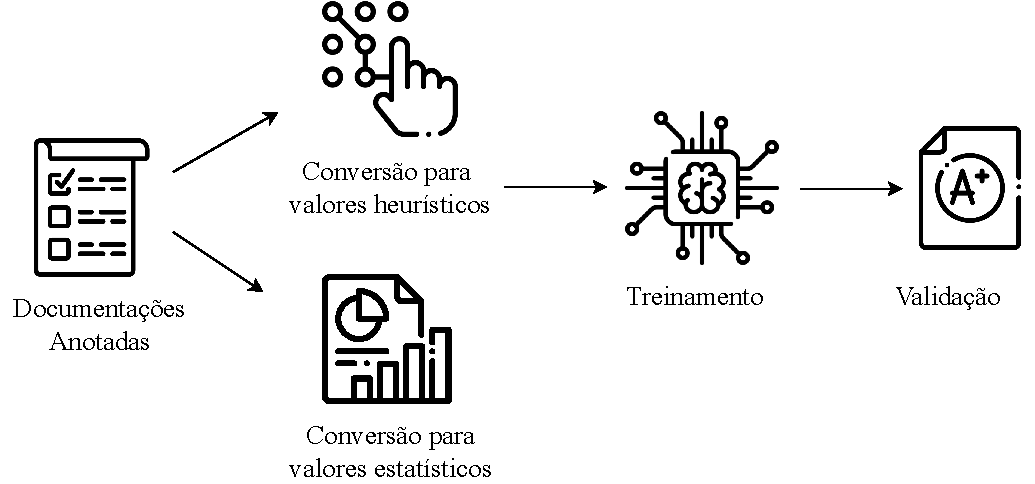
\includegraphics[width=0.8\textwidth]{figuras/metodo_classif.pdf}
    \caption[Construção do modelo de classificação]{Construção do modelo de classificação.}
    \label{fig:metodo-classif}
\end{figure}

\subsubsection{Preparação dos dados}
A preparação dos dados consistirá em dividir o conteúdo das planilhas entre características e rótulos para classificação. Neste estudo, consideraremos como características os parágrafos das planilhas analisadas pelos alunos, e rótulos as categorias que eles identificarem para cada um dos parágrafos. Como algoritmos de classificação só são capazes de compreender valores numéricos, os parágrafos serão convertidos em valores estatísticos e heurísticos. Serão considerados como valores estatísticos, características TF-IDF obtidas com o uso de bibliotecas de aprendizado de máquina. Já os valores heurísticos serão obtidos por meio de análise manual dos parágrafos e categorias marcadas. Quando um padrão linguístico que associe parágrafos a uma categoria for identificado pelo pesquisador, um novo valor heurístico será gerado como característica para classificação. 

A ideia de valores heurísticos emergiu do estudo realizado por \citet{prana2019categorizing}, que identificou, por exemplo, que o cabeçalho de uma documentação de um projeto poderia ser identificado pela ocorrência em texto do nome de seu repositório. Caso as características obtidas a partir destas duas estratégias não sejam suficientes, outras estratégias serão aplicadas nos dados obtidos a partir das planilhas. As marcações das categorias feitas pelos alunos serão convertidos em uma matriz binária de rótulos, seguindo a mesma estrutura disposta nas planilhas. Além da divisão entre rótulos e características para classificação, os valores convertidos também serão divididos em conjunto de treino e teste, a serem utilizados nas etapas seguintes.

\subsubsection{Treinamento}
A etapa de treinamento será responsável pela construção do modelo que identificará categorias relevantes a novatos em documentações de software livre. Como mais de uma categoria pode ocorrer para um mesmo trecho de documentação, classificadores multi-rótulos serão utilizados para treinamento dos algoritmos. Dado que a classificação multi-rótulos tende a ser mais complexa que outros tipos de aprendizagem, a estratégia de relevância binária será utilizada durante toda a etapa de treinamento. Na relevância binária, um problema de classificação com múltiplas classes como este, é transformado em problemas de classificação binária. Em outras palavras, o algoritmo de aprendizagem, ao invés de tentar identificar matematicamente todos as categorias de uma única vez nos trechos de documentação, tentará identifica-las separadamente, unindo os resultados ao final do processo. Esta é uma estratégia comumente utilizada por outros estudos que envolvam problemas multi-rótulos e classificação de textos. Durante o treinamento, o conjunto de treino será utilizado para alimentar os algoritmos de classificação.

Entre os algoritmos a serem treinados, se encontram: Random Forest (RF), Linear Support Vector Machine (SVM), Multinomial Naive Bayes (NB), K-Neighbors (kNN), Logistic Regression (LR), Multi-layer Perceptron (MLP), Linear Support Vector Machine + Stochastic Gradient Descent Learning (SGD). Estes algoritmos foram selecionados com base no que vem sendo utilizado por trabalhos relacionados, em especial, os estudos propostos por \citet{prana2019categorizing} e \citet{panichella2015how}. Além de trabalhos relacionados, os algoritmos MLP e SGD são recomendações propostas por desenvolvedores da Google\footnote{\url{https://developers.google.com/machine-learning/guides/text-classification/step-2-5}} e Scikit-learn\footnote{\url{https://scikit-learn.org/stable/tutorial/machine_learning_map/index.html}}, respectivamente.

\subsubsection{Validação}
Na etapa de validação, os modelos treinados serão avaliados a fim de se obter aquele que melhor identifique as categorias desejadas. Para isso, duas estrateǵias serão utilizadas, validação cruzada e métricas de acurácia. Na estratégia de validação cruzada, diversos conjuntos de treino e teste serão gerados a partir dos dados das planilhas, e estes serão avaliados por um algoritmo de validação \textit{k-fold} a fim de compreender se os modelos de classificação gerados são capazes de generalizar o problema desejado. Além da validação cruzada, métricas de acurácia serão utilizadas, em especial, \textit{precision}, \textit{recall} e \textit{f-measure}, todas amplamente conhecidas e utilizadas por demais trabalhos envolvendo problemas de classificação. Estas métricas irão avaliar utilizando os conjuntos de treino e teste a acurácia do classificador. O modelo que obtiver os melhores resultados será submetido a etapa de análise do classificador (Seção J).  

\subsection{Avaliação}
\label{sec:avaliacao}
Além do modelo de classificação, outras análises também serão entregues como parte dos resultados, entre elas, uma avaliação dos dados obtidos no experimento, e uma avaliação do modelo de classificação final.